\documentclass[10pt, a4paper]{scrartcl}

\usepackage{vorschule}
\usepackage[
	typ=ab,
	fach=Informatik,
	lerngruppe={Q2-GK},
	nummer=II.3,
	module={Symbole,Lizenzen},
	seitenzahlen=keine,
	farbig,
	lizenz=cc-by-nc-sa-4,
]{schule}

\usepackage[
	kuerzel=Ngb,
	reihe={Rechnernetze},
	version={2020-11-03},
]{ngbschule}

\author{J. Neugebauer}
\title{Topologie von Netzwerken}
\date{\Heute}

\setzeAufgabentemplate{ngbnormal}

\begin{document}
\ReiheTitel

Neben \emph{Gold City}, \emph{New Town}, \emph{Silver Lake} und \emph{Salt Lake} wollen auch die Orte \emph{Silver Spot}, \emph{Old Site}, \emph{Old Town} und \emph{Salt Village} in ein gemeinsames Kommunikationsnetz aufgenommen werden.

\begin{aufgabe}
Überlege dir zwei verschiedene Möglichkeiten, wie man aus dem bestehenden Netz ein gesamtes Netzwerk aufbauen könnte.

\begin{multicols}{2}
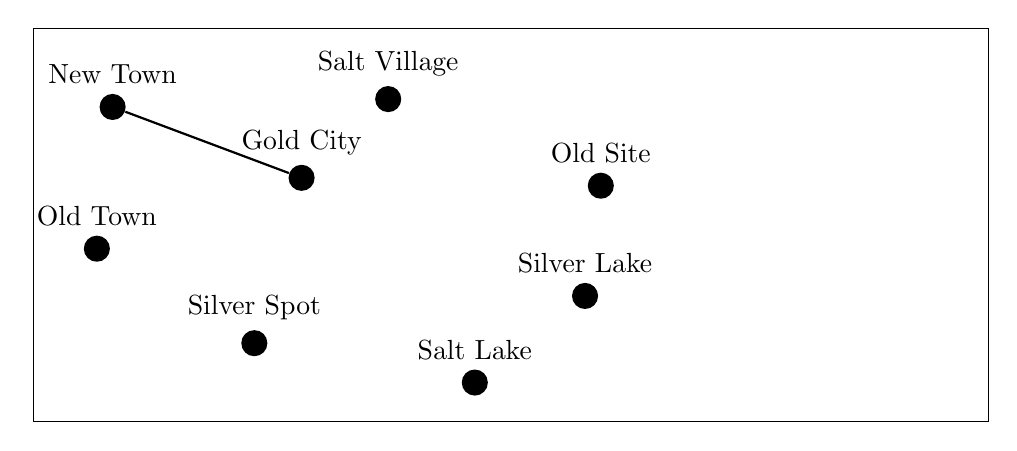
\begin{tikzpicture}
\draw (0,0) rectangle (\columnwidth,5);
\node[circle,fill=black,label={above:New Town}] at (1,4) (a) {};
\node[circle,fill=black,label={above:Gold City}] at (3.4,3.1) (b) {};
\draw[black,thick] (a) -- (b);

\node[circle,fill=black,label={above:Salt Village}] at (4.5,4.1) {};
\node[circle,fill=black,label={above:Old Site}] at (7.2,3) (b) {};
\node[circle,fill=black,label={above:Silver Lake}] at (7,1.6) (b) {};
\node[circle,fill=black,label={above:Salt Lake}] at (5.6,.5) (b) {};
\node[circle,fill=black,label={above:Silver Spot}] at (2.8,1) (b) {};
\node[circle,fill=black,label={above:Old Town}] at (.8,2.2) (b) {};
\end{tikzpicture}

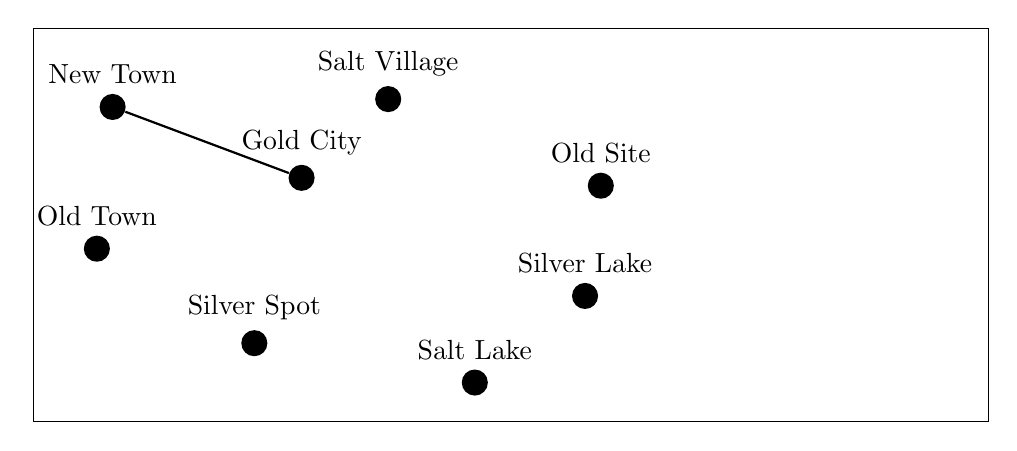
\begin{tikzpicture}
\draw (0,0) rectangle (\columnwidth,5);
\node[circle,fill=black,label={above:New Town}] at (1,4) (a) {};
\node[circle,fill=black,label={above:Gold City}] at (3.4,3.1) (b) {};
\draw[black,thick] (a) -- (b);

\node[circle,fill=black,label={above:Salt Village}] at (4.5,4.1) {};
\node[circle,fill=black,label={above:Old Site}] at (7.2,3) (b) {};
\node[circle,fill=black,label={above:Silver Lake}] at (7,1.6) (b) {};
\node[circle,fill=black,label={above:Salt Lake}] at (5.6,.5) (b) {};
\node[circle,fill=black,label={above:Silver Spot}] at (2.8,1) (b) {};
\node[circle,fill=black,label={above:Old Town}] at (.8,2.2) (b) {};
\end{tikzpicture}
\end{multicols}
\end{aufgabe}

\begin{aufgabe}
Den Aufbau eines \emph{Kommunikationsnetzwerks} nennt man eine \emph{Topologie}.

Stellt die Vor- und Nachteile deiner gezeichneten Netzwerktopologien tabellarisch gegenüber. Recherchiert dann im Internet nach weiteren Netzwerktopologien und ergänze die Tabelle um die neuen Topologien.

Welche Topologie hat sich im Internet durchgesetzt und warum?
\end{aufgabe}

\begin{aufgabe}
Erläutere die Begriffe:
\begin{itemize}
	\item Client-Server-Verbindung
	\item Peer-to-Peer-Verbindung
	\item Broadcast-Sendung
\end{itemize}
\end{aufgabe}

\begin{aufgabe}
Von \emph{New Town} soll eine Nachricht \enquote{Gold gefunden} nach \emph{Silver Lake} geschickt werden. Welche Informationen müssen dem \enquote{Datenpaket} hinzugefügt werden, damit eine sinnvolle Kommunikation zustande kommt?
\end{aufgabe}

\begin{aufgabe}
Die Übertragung von Datenpaketen geschieht im Internet über das \emph{TCP/IP-Protokoll}. Das Protokoll setzt sich zusammen aus dem \emph{Transmission Control Protocol} und dem \emph{Internet Protocol}.
	\begin{teilaufgaben}
		\teilaufgabe Recherchiere im Internet die Aufgabe des \emph{TCP}.
		\teilaufgabe Erläutere die Aufgabe und die Bestandteile des \emph{TCP-Headers}.
		\teilaufgabe Recherchiere im Internet die Aufgabe des \emph{IP}.
		\teilaufgabe Erläutere den Aufbau einer \emph{IP-Adresse} und einer \emph{Subnetzmaske}.
	\end{teilaufgaben}
\end{aufgabe}

\end{document}
